% Options for packages loaded elsewhere
\PassOptionsToPackage{unicode}{hyperref}
\PassOptionsToPackage{hyphens}{url}
%
\documentclass[
]{article}
\title{Rats : A normal hierarchical model}
\author{Vincent Guitteny, Freddie Joly, Tom Léchappé et Elyes Zribi}
\date{29 mars, 2022}

\usepackage{amsmath,amssymb}
\usepackage{lmodern}
\usepackage{iftex}
\ifPDFTeX
  \usepackage[T1]{fontenc}
  \usepackage[utf8]{inputenc}
  \usepackage{textcomp} % provide euro and other symbols
\else % if luatex or xetex
  \usepackage{unicode-math}
  \defaultfontfeatures{Scale=MatchLowercase}
  \defaultfontfeatures[\rmfamily]{Ligatures=TeX,Scale=1}
\fi
% Use upquote if available, for straight quotes in verbatim environments
\IfFileExists{upquote.sty}{\usepackage{upquote}}{}
\IfFileExists{microtype.sty}{% use microtype if available
  \usepackage[]{microtype}
  \UseMicrotypeSet[protrusion]{basicmath} % disable protrusion for tt fonts
}{}
\makeatletter
\@ifundefined{KOMAClassName}{% if non-KOMA class
  \IfFileExists{parskip.sty}{%
    \usepackage{parskip}
  }{% else
    \setlength{\parindent}{0pt}
    \setlength{\parskip}{6pt plus 2pt minus 1pt}}
}{% if KOMA class
  \KOMAoptions{parskip=half}}
\makeatother
\usepackage{xcolor}
\IfFileExists{xurl.sty}{\usepackage{xurl}}{} % add URL line breaks if available
\IfFileExists{bookmark.sty}{\usepackage{bookmark}}{\usepackage{hyperref}}
\hypersetup{
  pdftitle={Rats : A normal hierarchical model},
  pdfauthor={Vincent Guitteny, Freddie Joly, Tom Léchappé et Elyes Zribi},
  hidelinks,
  pdfcreator={LaTeX via pandoc}}
\urlstyle{same} % disable monospaced font for URLs
\usepackage[margin=1in]{geometry}
\usepackage{graphicx}
\makeatletter
\def\maxwidth{\ifdim\Gin@nat@width>\linewidth\linewidth\else\Gin@nat@width\fi}
\def\maxheight{\ifdim\Gin@nat@height>\textheight\textheight\else\Gin@nat@height\fi}
\makeatother
% Scale images if necessary, so that they will not overflow the page
% margins by default, and it is still possible to overwrite the defaults
% using explicit options in \includegraphics[width, height, ...]{}
\setkeys{Gin}{width=\maxwidth,height=\maxheight,keepaspectratio}
% Set default figure placement to htbp
\makeatletter
\def\fps@figure{htbp}
\makeatother
\setlength{\emergencystretch}{3em} % prevent overfull lines
\providecommand{\tightlist}{%
  \setlength{\itemsep}{0pt}\setlength{\parskip}{0pt}}
\setcounter{secnumdepth}{5}
\usepackage{stmaryrd} \usepackage{float} \floatplacement{figure}{H}
\ifLuaTeX
  \usepackage{selnolig}  % disable illegal ligatures
\fi

\begin{document}
\maketitle

\newenvironment{cols}[1][]{}{}
\newenvironment{col}[1]{\begin{minipage}{#1}\ignorespaces}{%
\end{minipage}
\ifhmode\unskip\fi
\aftergroup\useignorespacesandallpars}
\def\useignorespacesandallpars#1\ignorespaces\fi{%
#1\fi\ignorespacesandallpars}
\makeatletter
\def\ignorespacesandallpars{%
  \@ifnextchar\par
    {\expandafter\ignorespacesandallpars\@gobble}%
    {}%
}
\makeatother

\renewcommand\contentsname{Table des matières}
\newpage
\tableofcontents
\newpage

\hypertarget{pruxe9sentation-du-jeu-de-donnuxe9es}{%
\section{Présentation du jeu de
données}\label{pruxe9sentation-du-jeu-de-donnuxe9es}}

Nous disposons des poids de 30 jeunes rats, mesurés chaque semaine
pendant 5 semaines. La dimension de notre jeu de données est donc de 30
par 5. Nos variables \(x_j,j=1,…,5\) correspondent aux différents âges
des rats, en jour (\(x_j = {8,15,22,29,36}\)), et nos données \(Y_{ij}\)
correspondent au poids du rat \(i\) à l'âge \(x_j\).

Un tracé des 30 courbes de croissance suggère des signes de courbure
vers le bas :

\begin{center}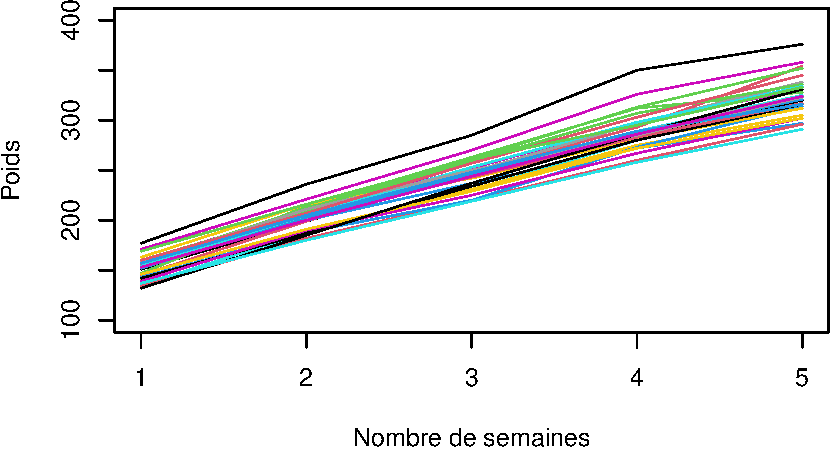
\includegraphics{Rats---A-normal-hierarchical-model_files/figure-latex/unnamed-chunk-1-1} \end{center}

\hypertarget{pruxe9sentation-du-moduxe8le}{%
\section{Présentation du modèle}\label{pruxe9sentation-du-moduxe8le}}

Le modèle est essentiellement une courbe de croissance linéaire à effets
aléatoires :

\(Y_{ij}\) \textasciitilde{}
\(\mathcal N(\alpha_i + \beta_i(x_j - \bar x), \sigma_c ^2)\) où
\(\bar x = 22\) et \(\sigma_c ^2\) \textasciitilde{}
\(InvGamma(a_c,b_c)\)

\(\alpha_i\) \textasciitilde{}
\(\mathcal N(\alpha_c,\sigma_{\alpha}^2)\)

\(\beta_i\) \textasciitilde{} \(\mathcal N(\beta_c,\sigma_{\beta}^2)\)

On note l'absence de paramètre représentant la corrélation entre
\(\alpha_i\) et \(\beta_i\). Pour l'instant, nous standardisons les
\(x_j\) autour de leur moyenne pour réduire la dépendance entre
\(\alpha_i\) et \(\beta_i\) dans leur vraisemblance : en fait, pour les
données entièrement équilibrées (centrées et réduites), une indépendance
complète est atteinte (notons qu'en général, l'indépendance a priori
n'oblige pas les distributions a posteriori à être indépendantes).

Les paramètres
\(\alpha_c, \sigma_{\alpha}^2, \beta_c, \sigma_{\beta}^2\) ont des loi a
priori « non informatives » et indépendantes :

\(\alpha_c\) \textasciitilde{} \(\mathcal N(0,\sigma_a^2)\)

\(\sigma_{\alpha}^2\) \textasciitilde{}
\(InvGamma(a_{\alpha},b_{\alpha})\)

\(\beta_c\) \textasciitilde{} \(\mathcal N(0,\sigma_b^2)\)

\(\sigma_{\beta}^2\) \textasciitilde{}
\(InvGamma(a_{\beta},b_{\beta})\).

\hypertarget{calculs-des-lois-a-posteriori}{%
\section{Calculs des lois a
posteriori}\label{calculs-des-lois-a-posteriori}}

\(\alpha_{c} \sim \mathcal{N}(O,\,\sigma_{a}^{2})\) ;
\(\alpha_{i} \sim \mathcal{N}(\alpha_{c},\,\sigma_{\alpha}^{2})\)

\begin{align*}
\Pi(\alpha_{c}|...) &\propto \Pi(\alpha_{c}) \prod_{i=1}^{n_{i}} \Pi(\alpha_{i}|\alpha_{c},\sigma_{\alpha}^{2} ) \\
        &\propto \exp\left(\frac{-\alpha_{c}^{2}}{2\sigma_{a}^{2}}\right)\prod_{i=1}^{n_{i}} \exp\left(\frac{-(\alpha_{i}-\alpha_{c})^{2}}{2\sigma_{\alpha}^{2}}\right) \\
        &\propto \exp\left(\frac{-\alpha_{c}^{2}}{2\sigma_{a}^{2}}\right)\prod_{i=1}^{n_{i}} \exp\left(\frac{-(\alpha_{c}^{2}-2\alpha_{i}\alpha_{c})}{2\sigma_{\alpha}^{2}}\right) \\
        &\propto \exp\left(\frac{-\alpha_{c}^{2}}{2\sigma_{a}^{2}}\right)\prod_{i=1}^{n_{i}} \exp\left(\frac{-ni\alpha_{c}^{2}+2\alpha_{c}\sum\limits_{i=1}^{n_{i}} \alpha_{i}}{2\sigma_{\alpha}^{2}}\right)\\
        &\propto \exp\left(\frac{-\alpha_{c}^{2}(\sigma_{\alpha}^{2}+ni\sigma_{a}^{2}) +2\alpha_{c}\sigma_{a}^{2}\sum\limits_{i=1}^{n_{i}} \alpha_{i}}{2\sigma_{a}^{2}\sigma_{\alpha}^{2}}\right)\\
        &\sim \mathcal{N}\left(\frac{\sigma_{a}^{2}\sum\limits_{i=1}^{n_{i}} \alpha_{i}}{\sigma_{\alpha}^{2}+n_{i}\sigma_{a}^{2}},\frac{\sigma_{a}^{2}\sigma_{\alpha}^{2}}{\sigma_{\alpha}^{2}+n_{i}\sigma_{a}^{2}}\right)
\end{align*}

\(\sigma_{\alpha}^{2} \sim InvGamma(a_{\alpha},b_{\alpha})\)

\begin{align}
\Pi(\sigma_{\alpha}^{2}|...) &\propto \Pi(\sigma_{\alpha}^{2}) \prod_{i=1}^{n_{i}}\Pi(\alpha_{i}|\alpha{c},\sigma_{\alpha}^{2}) \\
&\propto \exp^{\frac{-b_{\alpha}}{\sigma_{\alpha}^{2}}}(\sigma_{\alpha}^{2})^{-a_{\alpha}-1}\prod_{i=1}^{n_{i}} \exp\left(\frac{-(\alpha_{i}-\alpha_{c})^{2}}{2\sigma_{\alpha}^{2}}\right)(\sigma_{\alpha}^{2})^{-\frac{1}{2}}\\
&\propto (\sigma_{\alpha}^{2})^{-a_{\alpha}-1-\frac{n_{i}}{2}}\exp\left(\frac{-2b_{\alpha}-\sum\limits_{i=1}^{n_{i}}(\alpha_{i}-\alpha_{c})^{2}}{2\sigma_{\alpha}^{2}}\right)\\
&\sim InvGamma(\frac{n_{i}}{2}+a_{\alpha},\frac{+2b_{\alpha}+\sum\limits_{i=1}^{n_{i}}(\alpha_{i}-\alpha_{c})^{2}}{2})
\end{align}

\end{document}
